

\section{RESULT}
 
    \begin{table*}[tb]
        \centering
        \caption{Comparison of Variance Across Different Learning Conditions as Reflected in Table \ref{tab:COMPARISON RESULTS FOR THE LEARNING CONDITION}: A Detailed Analysis of Accuracies, F1 Scores, and AUC Metrics by Day and Model}
        \renewcommand{\arraystretch}{1.5}
        \resizebox{\linewidth}{3cm}{
        \begin{tabular}{|c|c|c|c|c|c|c|c|c|c|c|c|c|c|c|}
            \hline
            \multirow{2}{*}{Day} &\multirow{2}{*}{Evaluation} & \multicolumn{3}{c|}{TDV} & \multicolumn{3}{c|}{DDV} & \multicolumn{3}{c|}{TV} & \multicolumn{3}{c|}{SDTDV} & Random    \\
            \cline{3-15}
                        &            & EEG- Inception           & EEGNet                   & DevconvNet              & EEG- Inception             & EEGNet   & DevconvNet & EEG- Inception & EEGNet   & DevconvNet & EEG- Inception & EEGNet   & DevconvNet &          \\
            \hline
            \multirow{3}{*}{ Day 1} & Acc        & 7.25E-03                 & 9.21E-03                 & 9.21E-03                & 1.63E-02                   & 1.67E-03 & 1.35E-02   & 9.20E-03       & 5.04E-03 & 9.67E-04   & 1.10E-02       & 1.14E-02 & 1.04E-02   & 2.81E-07 \\
                                    & F1         & 1.71E-02                 & 1.99E-02                 & 1.99E-02                & 2.07E-02                   & 5.17E-03 & 2.24E-02   & 1.10E-02       & 7.80E-03 & 1.81E-01   & 1.37E-02       & 1.42E-02 & 1.47E-02   & 2.94E-07 \\
                                    & Auc        & 6.91E-03                 & 8.73E-03                 & 7.30E-02                & 6.20E-01                   & 1.46E-03 & 1.37E-02   & 9.21E-03       & 4.93E-03 & 5.17E-04   & 1.08E-02       & 1.17E+00 & 1.04E-02   & 2.83E-07 \\
            \hline
            \multirow{3}{*}{ Day 2} & Acc        & 1.24E-02                 & 1.50E-02                 & 4.40E-01                & 3.00E-01                   & 5.33E-03 & 1.89E-02   & 1.43E-02       & 7.09E-04 & 6.11E-04   & 1.27E-02       & 7.30E-03 & 6.07E-03   & 3.44E-07 \\
                                    & F1         & 2.06E-02                 & 2.34E-02                 & 1.47E-02                & 1.97E-02                   & 5.20E-03 & 3.05E-02   & 1.60E-02       & 1.73E-03 & 2.67E-03   & 1.43E-02       & 1.18E-02 & 9.40E-03   & 3.80E-07 \\
                                    & Auc        & 1.26E-02                 & 1.52E-02                 & 1.43E-02                & 1.81E-02                   & 5.29E-03 & 1.93E-02   & 1.43E-02       & 1.75E-04 & 6.68E-04   & 1.28E-02       & 7.36E-03 & 6.10E-03   & 3.43E-07 \\
            \hline
            \multirow{3}{*}{ Day 3} & Acc        & 1.26E-02                 & 8.19E-03                 & 7.86E-03                & 1.08E-02                   & 3.37E-03 & 2.27E-02   & 1.28E-02       & 1.60E-02 & 1.20E+00   & 1.29E-02       & 7.99E-03 & 1.04E-02   & 2.85E-07 \\
                                    & F1         & 1.99E-02                 & 1.02E-02                 & 1.59E-02                & 1.47E-02                   & 3.64E-03 & 2.41E-02   & 1.31E-02       & 1.92E-02 & 1.30E-02   & 1.45E-02       & 1.53E-02 & 1.30E-02   & 3.75E-07 \\
                                    & Auc        & 1.44E-02                 & 8.47E-03                 & 7.29E-03                & 1.01E-02                   & 3.09E-03 & 2.23E-02   & 1.29E-02       & 1.60E-02 & 1.19E-02   & 1.32E-02       & 7.93E-03 & 1.00E-02   & 2.79E-07 \\
            \hline
            \multirow{3}{*}{ Day 4} & Acc        & 1.68E-02                 & 1.40E-02                 & 1.78E-02                & 2.04E-02                   & 1.56E-03 & 2.22E-02   & 1.13E-02       & 2.99E-03 & 1.50E-03   & 2.18E-02       & 1.13E-02 & 1.70E-02   & 2.26E-07 \\
                                    & F1         & 2.49E-02                 & 1.71E-02                 & 3.09E-02                & 2.28E-02                   & 3.04E-03 & 2.64E-02   & 1.45E-02       & 6.26E-03 & 1.74E-02   & 2.45E-02       & 1.97E-02 & 2.50E-02   & 2.37E-07 \\
                                    & Auc        & 1.70E-02                 & 1.41E-02                 & 1.78E-02                & 2.03E-02                   & 1.37E-03 & 2.21E-02   & 1.13E-02       & 2.58E-03 & 1.47E-02   & 2.20E-02       & 1.14E-02 & 1.78E-02   & 2.26E-07 \\
            \hline
            \multirow{3}{*}{ Day 5} & Acc        & 1.77E-02                 & 1.32E-02                 & 1.80E-02                & 1.71E-02                   & 1.49E-02 & 2.06E-02   & 1.56E-02       & 1.70E-02 & 2.06E-02   & 1.57E-02       & 1.34E-02 & 1.70E-02   & 3.35E-07 \\
                                    & F1         & 1.85E-02                 & 2.55E-02                 & 2.02E-02                & 2.58E-02                   & 2.98E-02 & 2.67E-02   & 2.07E-02       & 1.90E-02 & 2.79E-02   & 1.95E-02       & 1.40E-02 & 2.70E-02   & 6.20E-07 \\
                                    & Auc        & 1.77E-02                 & 1.28E-02                 & 1.78E-02                & 1.72E-02                   & 1.45E-02 & 2.03E-02   & 1.50E-02       & 1.70E-02 & 1.98E-02   & 1.52E-02       & 1.34E-02 & 1.58E-02   & 3.40E-07 \\
            \hline
        \end{tabular}}

        \label{tab:VARIANCE COMPARISON}
    \end{table*}
    
    
  \begin{table*}[tb]
      \centering
      \caption{Comparison of methods using Bayesian analysis of variance for f1 scores.}
      \label{table:Comparison of methods using Bayesian analysis of variance for f1 scores.}
      \begin{tabular}{|l|r|r|r|r|r|r|r|r|}
          \hline
          Parameter        & SD     & hdi\_3\% & hdi\_97\% & mcse\_mean & mcse\_sd & ess\_bulk & ess\_tail & r\_hat \\
          \hline
          TDV means        & 0.520  & 0.014    & 0.495     & 0.545      & 0.0      & 0.0       & 5346.0    & 2678.0 \\
          \hline
          DDV means        & 0.551  & 0.014    & 0.526     & 0.577      & 0.0      & 0.0       & 4729.0    & 3310.0 \\
          \hline
          TV means         & 0.550  & 0.011    & 0.528     & 0.570      & 0.0      & 0.0       & 6730.0    & 3418.0 \\
          \hline
          SDTDV means      & 0.560  & 0.012    & 0.537     & 0.581      & 0.0      & 0.0       & 5050.0    & 3424.0 \\
          \hline
          TDV sigmas       & 0.151  & 0.010    & 0.132     & 0.169      & 0.0      & 0.0       & 5694.0    & 2888.0 \\
          \hline
          DDV sigmas       & 0.152  & 0.010    & 0.133     & 0.170      & 0.0      & 0.0       & 5054.0    & 3118.0 \\
          \hline
          TV sigmas        & 0.126  & 0.008    & 0.112     & 0.143      & 0.0      & 0.0       & 4897.0    & 2734.0 \\
          \hline
          SDTDV sigmas     & 0.133  & 0.008    & 0.118     & 0.149      & 0.0      & 0.0       & 4119.0    & 2925.0 \\
          \hline
          TDV diff\_means  & -0.026 & 0.012    & -0.048    & -0.004     & 0.0      & 0.0       & 5155.0    & 3023.0 \\
          \hline
          DDV diff\_means  & 0.006  & 0.012    & -0.016    & 0.027      & 0.0      & 0.0       & 4891.0    & 3131.0 \\
          \hline
          TV diff\_means   & 0.005  & 0.010    & -0.014    & 0.024      & 0.0      & 0.0       & 6416.0    & 3254.0 \\
          \hline
          SDTV diff\_means & 0.014  & 0.010    & -0.007    & 0.033      & 0.0      & 0.0       & 5120.0    & 3251.0 \\
          \hline
      \end{tabular} 
  \end{table*}
  
   \begin{table*}[tb]
    \centering
    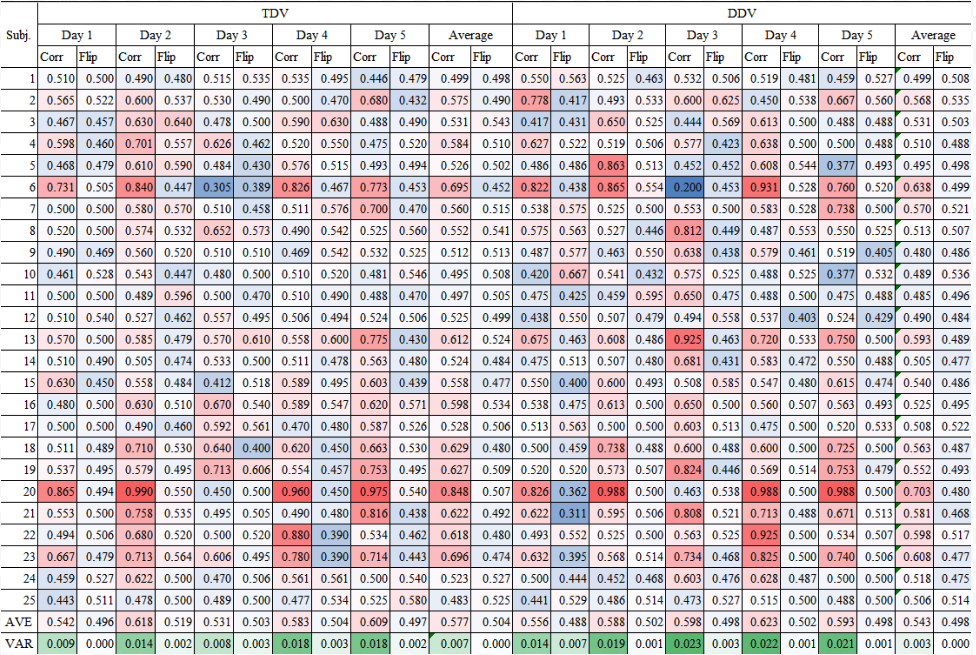
\includegraphics[width=\linewidth]{Flipdata.png}
    \caption{Learning with correct labels and learning with reversed labels for TDV and DDV EEGInception}
    \label{tab: Learning with correct labels and learning with reversed labels for TDV and DDV EEGInception}
    \end{table*}
    \subsection{Performance of the Proposed Verification Techniques}
    The analysis of TABLE\ref{tab:COMPARISON RESULTS FOR THE LEARNING CONDITION} offers a comprehensive understanding of the effectiveness of different learning conditions in EEG-based model training. The table compares five distinct approaches: TDV, DDV, TV, SDTDV, and a Random model across multiple metrics - Accuracy (Acc), F1-Score (F1), and Area Under Curve (Auc) - over a span of five days and an overall average.

    TDV approach shows moderate success. It consistently outperforms the Random model, suggesting the efficacy of pre-training on historical EEG data. However, when compared to other models, particularly DDV and SDTDV, its performance is not the most outstanding.
        
    DDV approach evident in its generally higher scores across all metrics, particularly on the fourth day. This suggests that including a small portion of test-day data can significantly boost the model's real-time identification accuracy. The highest numbers for ACC, F1-score, and AUC are colored pink.
        
    TV approach, which relies solely on test-day data, demonstrates a notable performance, especially in Accuracy and Auc metrics. This indicates that for certain applications, immediate day training without historical data might be sufficient, offering a more streamlined approach.
    
   SDTDV takes a more personalized approach, using only the subject's historical data for pre-training. This method's performance, particularly in Accuracy and F1-Score, is generally on par with TDV, indicating that individualized training does have merit, although it may not significantly outperform more generalized approaches.
    \vspace{1mm}
    \subsection{EEG Model Showdown: EEGInception Reigns Supreme}
    \vspace{1mm}
    Fig. \ref{fig: Each model for each validation}, \ref{fig: Each evaluation  for each validation} shows the classification accuracy (Acc), F1 score (F1), and area under the curve (AUC) are visualized. Boxplots are useful for showing the distribution, median, quartiles, and outliers of your data. The line in the middle of the box represents the median, the top and bottom edges of the box represent the third and first quartiles, respectively, and the whiskers are typically 1.5 times the interquartile range from the top and bottom quartiles. Indicates up to the outer data point. If a data point falls outside this range, it will be plotted as an outlier.
    
    
    \subsubsection{EEG Model Showdown: EEGInception Reigns Supreme}
    Key points discernible from Fig. \ref{fig: Each model for each validation} indicate that the performance of models across different validation sets is not consistent, and certain models may excel in specific validation sets. For instance, the Dev2Net model shows higher performance in the TDV and DDV validation sets but has smaller differences in others. On the other hand, EEGInception and EEGNet exhibit relatively stable performance, though not markedly superior in specific metrics or validation sets.
    
    \begin{itemize}
        \vspace{1mm}
      \item \textbf{EEGInception}: EEGInception model potentially exhibits a relatively narrow interquartile range, suggesting that the model provides consistent performance across various validation sets. It is expected to demonstrate stable performance, particularly on standardized datasets (TDV, DDV, TV), indicating EEGInception's adaptability to data with different characteristics and implying high generalization ability.
      \vspace{3mm}
      \item \textbf{EEGNet}: EEGNet model might show tendencies of wider interquartile ranges in specific validation sets, indicating sensitivity to specific data characteristics or significant performance variability under certain conditions. Performance instability in the DDV set could be anticipated, potentially reflecting the model's sensitivity to different data distributions. The breadth of EEGNet's interquartile range implies the necessity of caution in the model's adjustment or application.
      \vspace{3mm}
      \item \textbf{Dev2Net}: Dev2Net model demonstrates good performance in TDV and DDV sets, the possibility of wider interquartile ranges compared to other models suggests potential significant performance variability under some conditions. This might indicate that Dev2Net can achieve high performance but is strongly dependent on the characteristics of specific datasets. Significant variability in metrics like F1 score or AUC could reflect the model's sensitivity to the balance between different classes or the identification of specific classes.
    \end{itemize}


    \subsubsection{Dependency of Model Performance on Validation Method}

    From Fig. \ref{fig: Each evaluation  for each validation}, it is evident that there is a significant difference in the distribution of scores across various validation methods and models, indicating that model performance is contingent upon the validation method employed. Some models demonstrate high accuracy, F1 scores, and AUC in certain validation methods while underperforming in others, highlighting the influence of validation methodologies on model efficacy. The consistency of scores in Random validation (around 0.5) suggests its role as a baseline.

    Fluctuation in model performance across different validation methods may suggest that certain models are more apt for specific types of data or problem configurations. For instance, the EEGInception model consistently outperforms others in TDV and DDV validations but not in TV validation, suggesting its enhanced capability to capture certain data characteristics or its effective regularization against overfitting in specific contexts. Conversely, the Dev2Net model exhibits stable performance in TDV and DDV, occasionally surpassing other models in AUC, indicating its potential superior generalizability across diverse datasets and problem settings.
    \begin{itemize}
        \vspace{1mm}
        \item \textbf{TDV}: Relatively wide interquartile range (IQR) observed for the Dev2Net model in TDV might indicate its high adaptability to training data without directly translating to consistent performance improvement. In contrast, a narrower IQR for the EEGInception model implies its stable performance on training data.
        \vspace{3mm}
        \item \textbf{DDV}: In DDV, the IQR, especially for the EEGInception and Dev2Net models, reflects their capability to adapt to different data characteristics. A narrow IQR for EEGInception suggests its ability to maintain stable performance across various datasets, while a wide IQR for Dev2Net indicates potential performance variability.
        \vspace{3mm}
        \item \textbf{TV}: Breadth of the IQR in TV validation acts as an indicator of a model's generalization ability to test data, where a wider IQR suggests potential instability in performance on unfamiliar data. This is particularly relevant for the EEGNet model, which may show considerable performance variability across different testing scenarios.
        \vspace{3mm}
        \item \textbf{SDTDV}: Validation through SDTDV is advantageous for minimizing accuracy variance. The analysis of the IQR in SDTDV allows for the assessment of a model's adaptability to semi-diverse training data. A narrow IQR indicates that a model consistently performs well on such data. EEGInception and Dev2Net displaying a relatively narrow IQR suggests their capability to maintain stable performance across semi-diverse datasets.
    \end{itemize}
    \vspace{1mm}
    
    \subsection{Daily variations in learning conditions and comparisons between models in EEG analysis }
    Table \ref{tab:VARIANCE COMPARISON} summarises the analysis of EEG data under different learning conditions. Several EEG analysis models, including EEG-Inception, EEGNet, and DevconvNet, were used to assess the variability of subjects' performance.

    Table \ref{tab:VARIANCE COMPARISON} presents the values of 'Acc (Accuracy)', 'F1 (F1 score)', and 'Auc (area under the curve)' for each day, indicating considerable variability in model performance from day to day. It is important to note that certain models have different accuracy and F1 scores between 'Day 1' and 'Day 3', indicating that training conditions and subject responses may vary day to day.
    
    When comparing different models, each one performs better on specific assessment measures. 'EEG-Inception' and 'DevconvNet' have higher 'Auc' values on some days, suggesting that these models may have better discriminative ability under certain conditions.
    
    
    \subsection{Comparison of methods by Bayesian analysis of variance}
    Table \ref{table:Comparison of methods using Bayesian analysis of variance for f1 scores.} compares four methods: TDV, DDV, TV, and SDTDV, using Bayesian analysis of variance. The means of each method are 0.520, 0.551, 0.550, and 0.560, respectively, with SDTDV having the highest mean value. However, this difference is not significant compared to the other methods. It is important to note that all methods have similar means and should be considered equally effective. Therefore, this result suggests that SDTDV is not significantly superior to the other methods.

    A comparison of standard deviations was conducted. The standard deviations for TDV, DDV, TV and SDTDV are 0.151, 0.152, 0.126 and 0.133 respectively. This shows that TV has the lowest standard deviation, indicating that it is more consistent in its results than the other methods.

    The mean difference between the methods reveals that TDV has the smallest difference at -0.026. DDV, TV, and SDTDV have differences close to zero, suggesting that their means are similar. This result indicates that all methods perform similarly.

     Additionally, we examine the ESS and r\_hat values, which serve as indicators of the quality of Bayesian analysis. The high ESS values and r\_hat values close to 1 for all methods indicate good model convergence. The analysis results are highly reliable.

    TV shows the best results compared to other methods, with the lowest standard deviation indicating high consistency. However, the other methods also have small performance differences, so it is important to select the appropriate method depending on the purpose and situation. The analysis is highly reliable, as evidenced by the high ESS values and r\_hat values close to 1 obtained for all methods.
    \subsection{Some subjects are more accurate when labels are reversed}
    Table \ref{tab: Learning with correct labels and learning with reversed labels for TDV and DDV EEGInception} compares learning with correct labels and learning with reversed labels for TDV and DDV EEGInception, by day of the week and by subject. The desired result of inverted-labels learning should be a recognition result of less than 50\% in almost all cases, but in reality, identification is performed with an average of 50\% and microscopic variation. As the labels are learnt by inverting the labels, this would normally have to be below the accuracy of normal learning in all subjects. Some subjects tend to show an average of 53\% agreement over a five-day period, even when learning opposite labels. Some have exceeded the accuracy of learning the labels inverted. This phenomenon suggests that some subjects may be presenting opposite signals based on the general EEG tendencies of other subjects.